% Section content template for individual Educative lessons
% This file contains the actual content for a specific section
% Generated from Educative API section content

% Section: Creational Design Patterns
% Section ID: 6512418782183424
% Section Slug: creational-design-patterns
% Generated: 2025-12-11T06:15:51.881089

\subsection{Introduction to creational design patterns}\label{introduction-to-creational-design-patterns}
\\
In this lesson, we will discuss creational design patterns. \textbf{Creational design patterns} deal with object creation mechanisms. As the name implies, these patterns provide optimized object creation techniques. They help cater to the design and complexity problems that might occur when using the basic approach. They also help control the creation of objects.
\\
The chart below shows the patterns that fall under this category:

\begin{figure}[htbp]
 \centering
 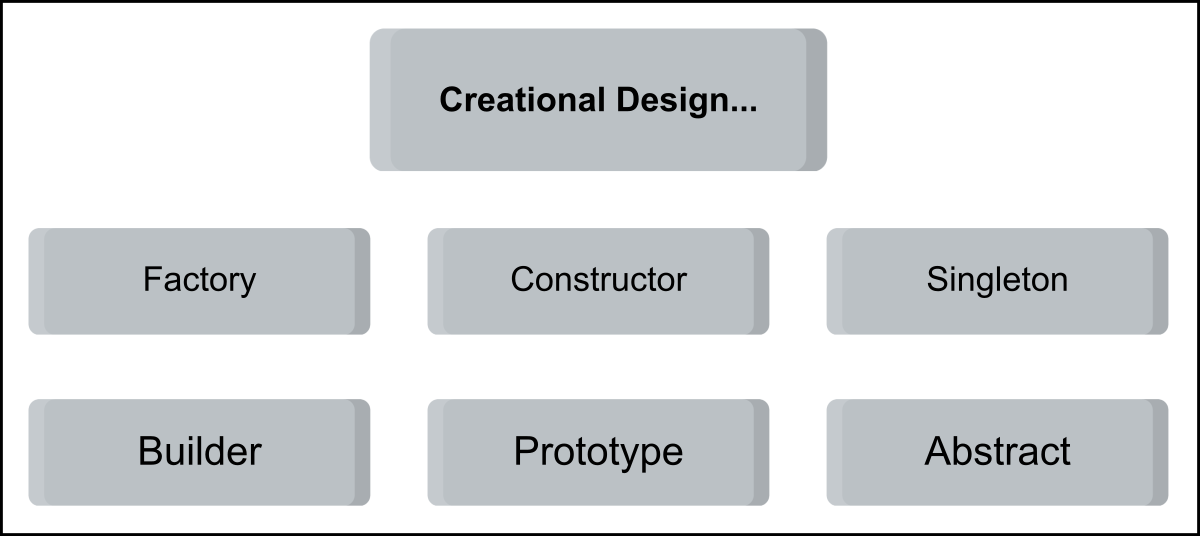
\includegraphics[width=0.5\textwidth]{Images/chapter_5/section_6512418782183424/6614187059183616.png}
 \caption{Creational design patterns}
\end{figure}

\subsubsection{Factory pattern}\label{factory-pattern}
\\
The \textbf{Factory pattern} is a creational pattern that provides a template that can be used to create objects. It is used in complex situations where the type of the object required varies and needs to be specified in each case.
\\
It does not use the \texttt{new} keyword directly to instantiate objects. This means that it does not explicitly require the use of a constructor to create objects. Instead , it provides a generic interface that delegates the object creation responsibility to the corresponding subclass.

\subsubsection{Constructor pattern}\label{constructor-pattern}
\\
The \textbf{Constructor pattern}, as the name defines, is a class-based pattern that uses the constructors present in the class to create specific types of objects.

\subsubsection{Singleton pattern}\label{singleton-pattern}
\\
The \textbf{Singleton pattern} is a type of design pattern that restricts the instantiation of a class to a single object. This allows the class to create its instance the first time it is instantiated. However, on the next try, the existing instance of the class is returned. No new instance is created.

\subsubsection{Builder pattern}\label{builder-pattern}
\\
The Builder pattern is a type of a creational design pattern that helps in building complex objects using simpler objects. It provides a flexible and step-by-step approach towards making these objects. It also shields the representation and process of creation.

\subsubsection{Prototype pattern}\label{prototype-pattern}
\\
The \textbf{Prototype pattern} is used to instantiate objects with some default values using an existing object. It clones the object and provides the existing properties to the cloned object using prototypal inheritance.
\\
In \textbf{prototypal inheritance}, a prototype object acts as a blueprint from which other objects inherit when the constructor instantiates them. Hence, any properties defined on the prototype of a constructor function will also be present in the cloned object it creates.

\subsubsection{Abstract pattern}\label{abstract-pattern}
\\
We use the Factory pattern to create multiple objects from the same family without having to deal with the creation process. The \textbf{Abstract pattern} is similar. The difference is that it provides a constructor to create families of related objects. It is abstract, which means that it does not specify concrete classes or constructors.

\textbf{When to use creational design patterns?}

\begin{table}[htbp]
\centering
\small
\adjustbox{max width=\textwidth}{
\begin{tabular}{|p{0.221\textwidth}|p{0.729\textwidth}|}
\hline
\textbf{Creational Design Patterns} & \textbf{When to use} \\
\hline
\hline
\hfill\break \hfill\break Factory pattern & \begin{itemize} \tightlist \item When the type of objects required cannot be anticipated beforehand. \item When multiple objects that share similar characteristics need to be created. \item When you want to generalize the object instantiation process, since the object set up is complex in nature. \end{itemize} \hfill\break \\
\hline
\hfill\break \hfill\break Constructor pattern & \begin{itemize} \tightlist \item You can use it when you want to create multiple instances of the same template, since the instances can share methods but can still be different.~ \item It can be useful in the Libraries and Plugins design. \end{itemize} \hfill\break \\
\hline
\hfill\break \hfill\break \hfill\break \hfill\break Singleton pattern & \begin{itemize} \tightlist \item The Singleton pattern is mostly used in cases where we want a single object to coordinate actions across a system. \item \textbf{Services} can be singleton since they store the state, configuration, and provide access to resources. Therefore, it makes sense to have a single instance of a service in an application. \item \textbf{Databases} such as MongoDB utilize the Singleton pattern when it comes to database connections. \item \textbf{Configurations} are used if there is an object with a specific configuration, and we don't need a new instance every time that configuration object is needed. \end{itemize} \hfill\break \\
\hline
\hfill\break \hfill\break Builder pattern & \begin{itemize} \tightlist \item You can use this design pattern when building apps that require you to create complex objects. It can help you hide the construction process of building these objects. \item A good example would be a DOM, where we might need to create plenty of nodes and attributes. The construction process can get quite messy if we are building a complex DOM object. In cases like these, the Builder pattern can be used. \end{itemize} \\
\hline
\hfill\break Prototype pattern & \begin{itemize} \tightlist \item To eliminate the overhead of initializing an object. \item When we want the system to be independent about how the products in it are created. \item When creating objects from a database whose values are copied to the cloned object. \end{itemize} \\
\hline
\hfill\break \hfill\break Abstract pattern & \begin{itemize} \tightlist \item Applications requiring the reuse or sharing of objects. \item Applications with complex logic because they have multiple families of related objects that need to be used together. \item When we require object caching. \item When the object creation process is to be shielded from the client. \end{itemize} \\
\hline
\end{tabular}
}
\caption{When to use creational design patterns?}
\end{table}

Let's look at the structural design patterns in the next lesson.

% End of section content